Een lamp of een andere elektronisch apparaat wil je uit en aan kunnen zetten. Dat schakelen doen we met een schakelaar (Engels: switch)\index{Schakelaar}\index{Switch}.

In de elektronica wordt een switch weergegeven met het symbool dat je ziet weergegeven in \ref{symbool:switch}

\begin{figure}[h]
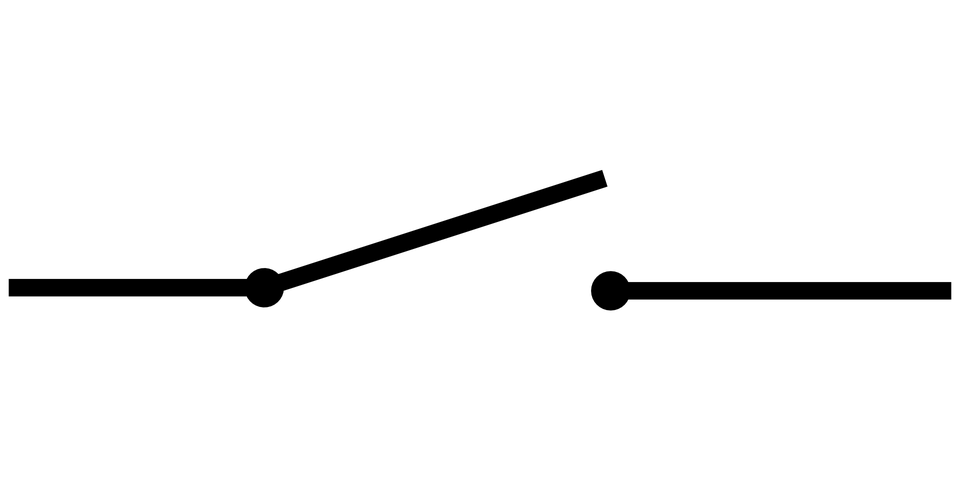
\includegraphics[width=5cm]{switch}
\centering
\caption{Symbool van een schakelaar}
\label{symbool:switch}
\end{figure}

Er zijn verschillende soorten schakelaars en toch zal je over het algemeen alleen het weergegeven symbool voor de schakelaar tegen komen.
